%!TEX root = ../document.tex

\section{User Testing and Feedback}
\label{sec:USER_TESTING}

For testing our paper prototype we interviewed the students from both bachelor's projects at the EPIC chair. (Figure  \ref{fig:user_testing}) They are developing applications based on SAP's HANA technology and are also facing the problems we discovered during our external interviews. The first Team (HP1) investigates In-Memory Data Management for Enhanced ERP while the other (HP2) focuses on Real-time Analysis of Genome Data.

\begin{figure}
\begin{centering}
    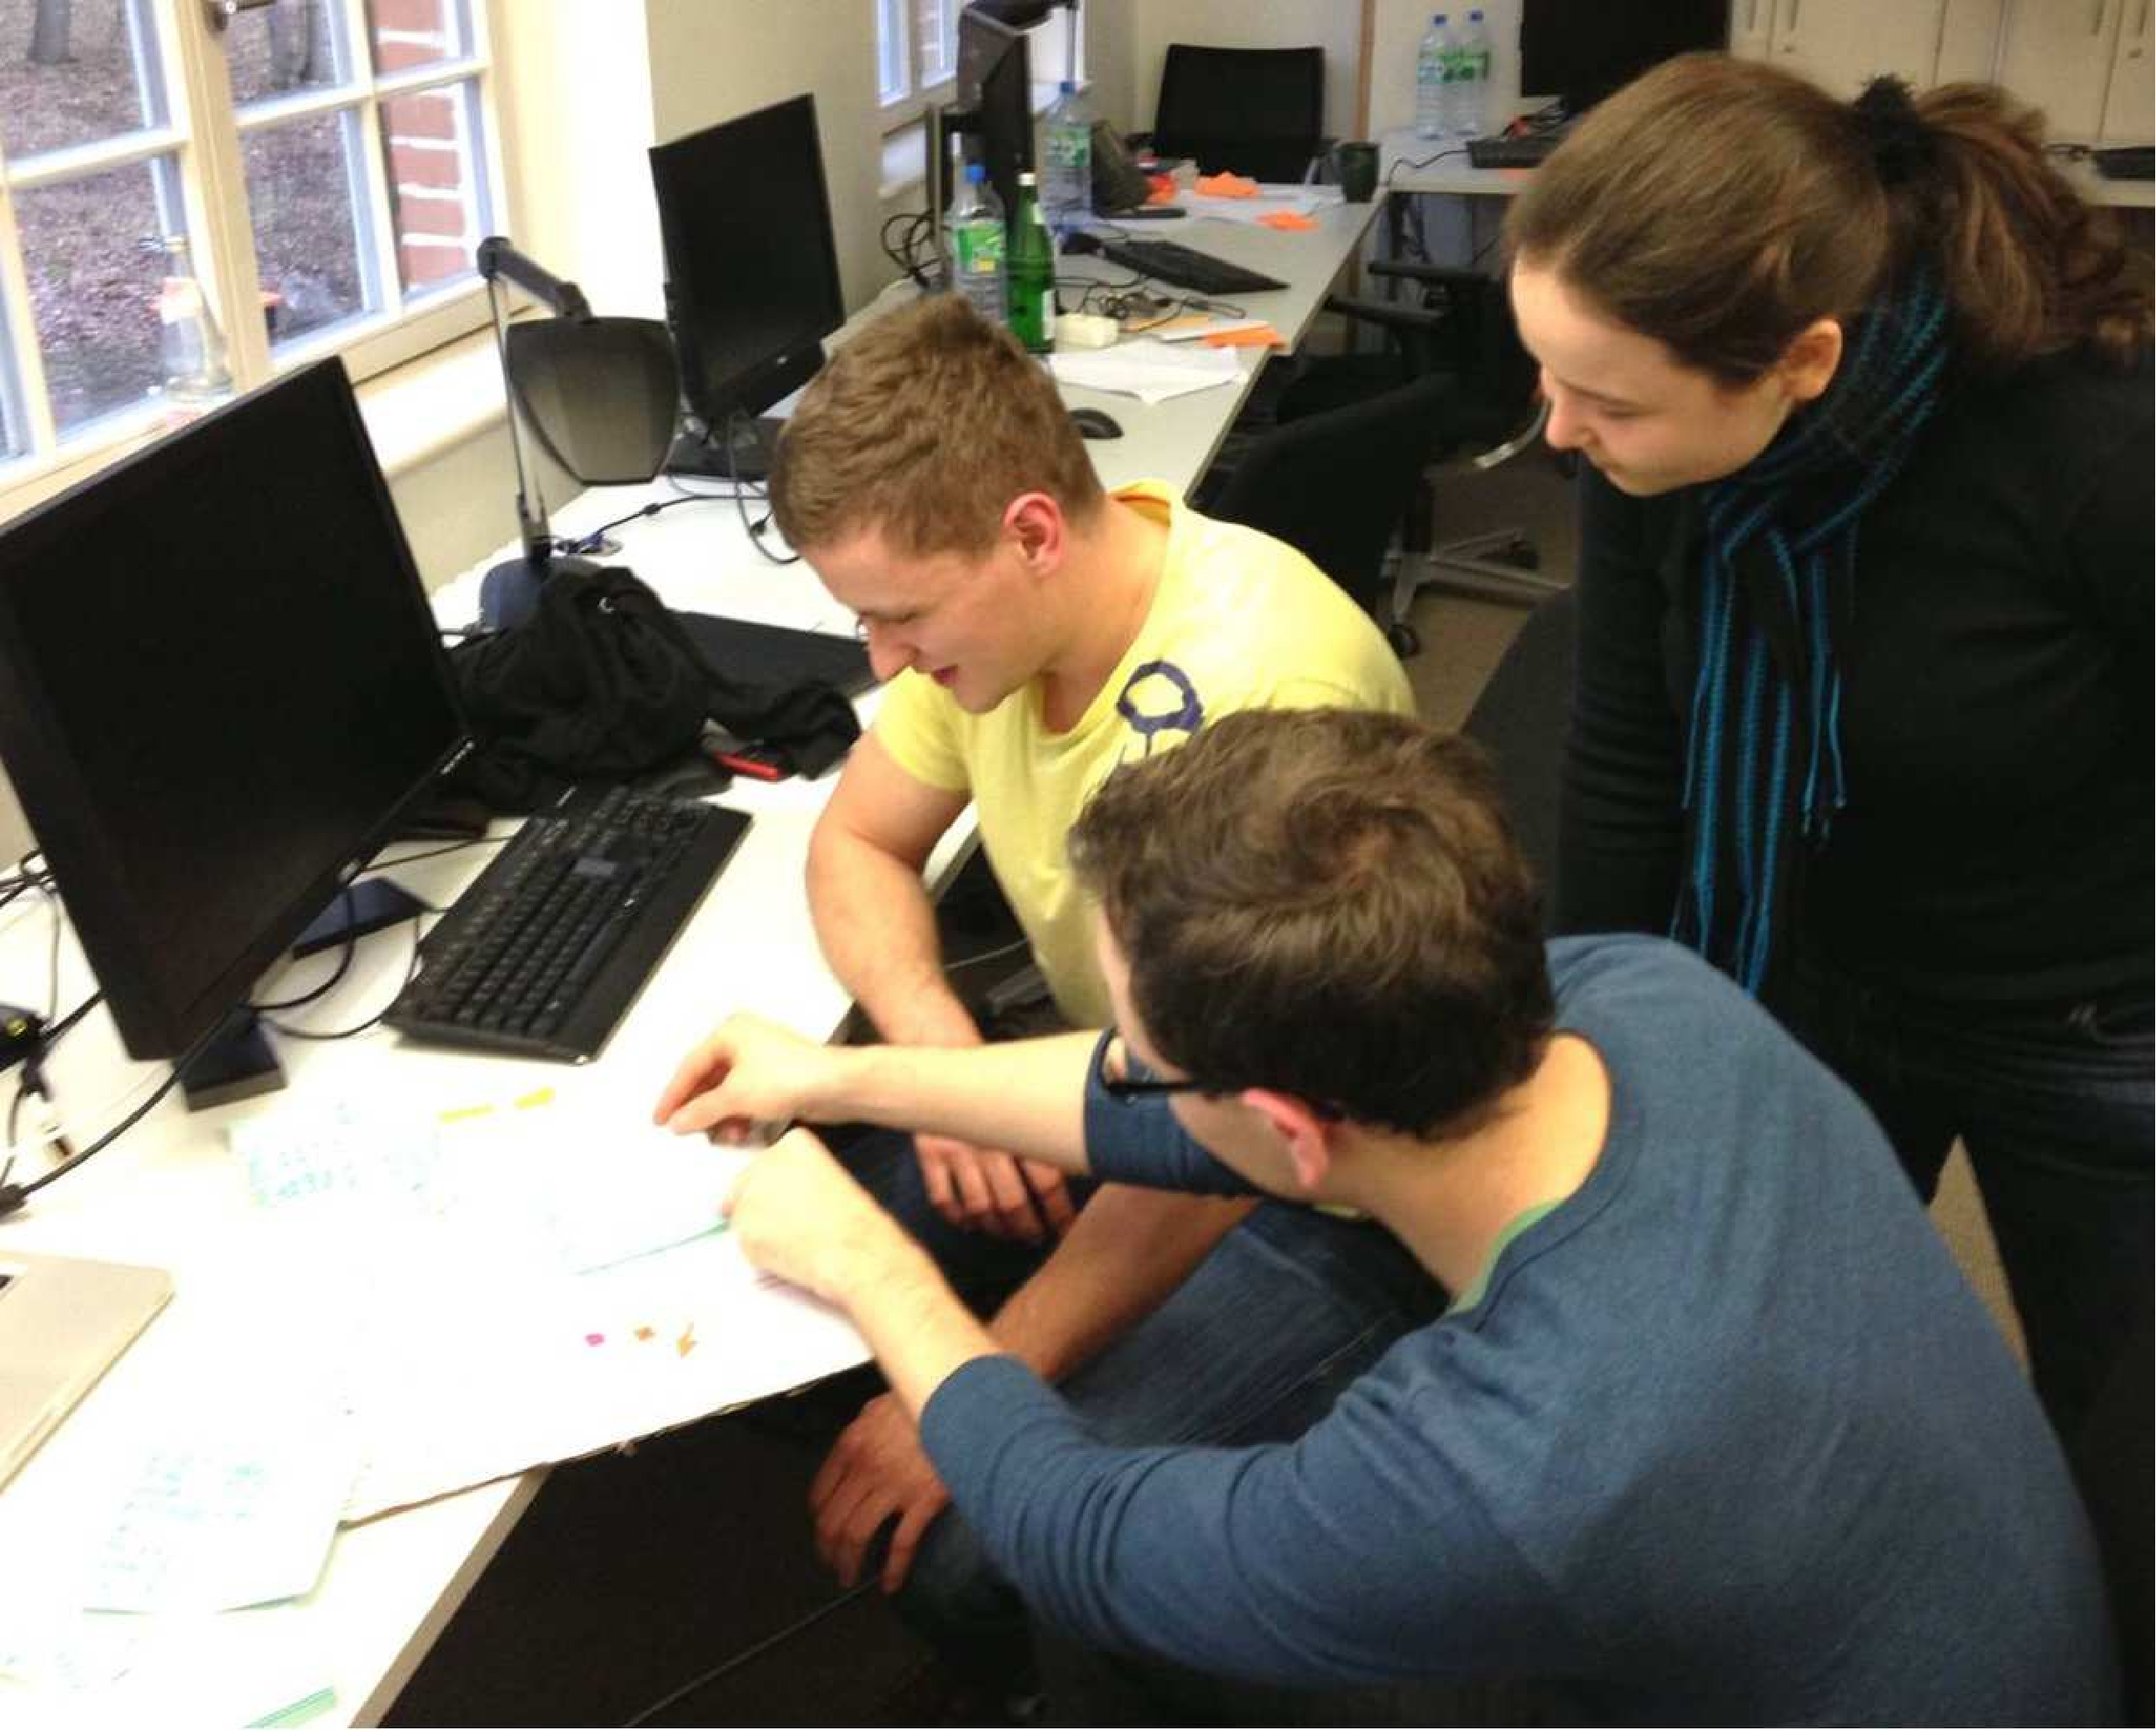
\includegraphics[width=1.0\linewidth]{images/user_testing}
    \caption{User testing with the Bachelor's project team HP2}
    % #selfrespect
    \label{fig:user_testing}
\end{centering}
\end{figure}

In the following we present their feedback as well as general insights we gained during the workshop week from Hasso Plattner and some of the tutors.

\subsection{Feedback from Bachelor's Project HP1}
\label{subsec:FeedbackBPHP1}
\begin{itemize}
	\item Popups are nice, but they occlude the underlying code. Even if they would be detachable and could be positioned freely on the screen, this would lead to a cluttered workspace and thus result in an inferior workspace.

	\item For maximum productivity they would rather use keyboard shortcuts instead of clicking with your mouse on the data entitites in the code.

	\item Screen real estate is important for developers, even on todays large screen monitors. So, we should keep that in mind while providing more and more information of the underlying data context.
\end{itemize}

\subsection{Feedback from Bachelor's Project HP2}
\label{subsec:FeedbackBPHP2}
\begin{itemize}
	\item The concept of a data context is hard to grasp when presented initially.

	\item They liked the immediate feedback in the context panel and appearing warnings or hints next to a context, if some of their code changes result in unintended behaviour on other contexts.

	\item The context panel should also include all relevant test cases, so they do not need any additional testing tools to run their test suite.
\end{itemize}


\subsection{General Feedback during the week}
\label{subsec:FeedbackWeek}
	MISSING

\subsection{Feedback evaluation}
\label{subsec:FeedbackEvaluation}
	MISSING


\begin{figure}
\begin{centering}
    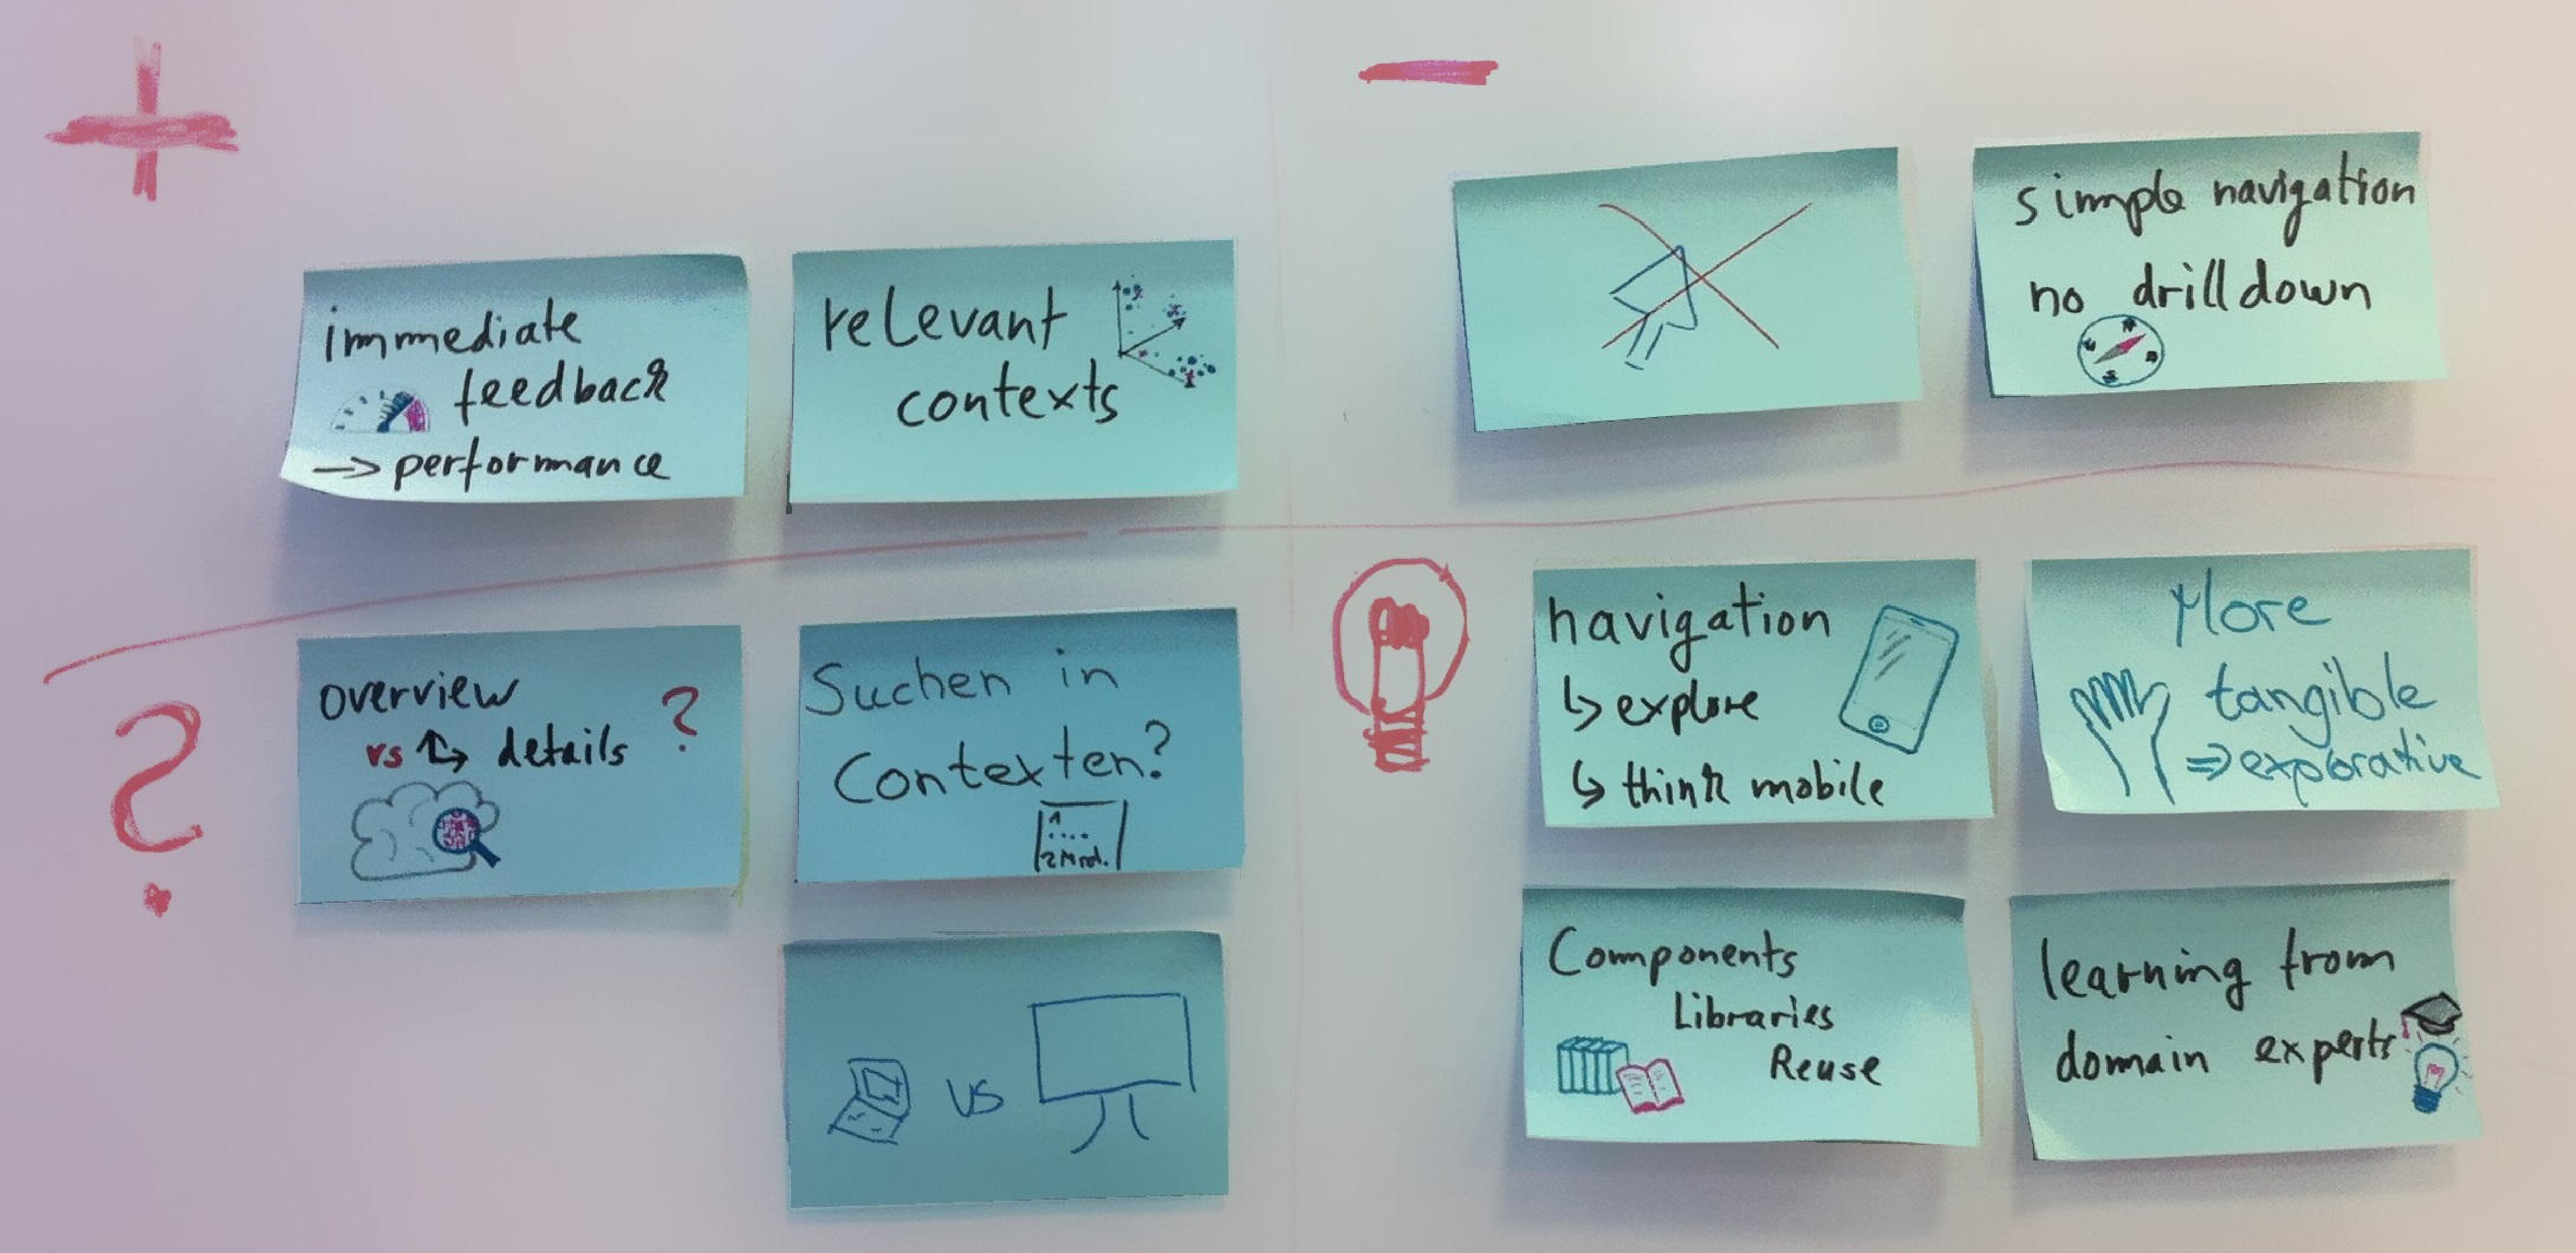
\includegraphics[width=1.0\linewidth]{images/user_feedback}
    \caption{User feedback captured on Post-Its and arranged in the feedback panel with positive and negative feedback as well as questions and new ideas}
    % #selfrespect
    \label{fig:user_feedback}
\end{centering}
\end{figure}